\begingroup
\usetikzlibrary{positioning}
\fontfamily{cmss}\selectfont
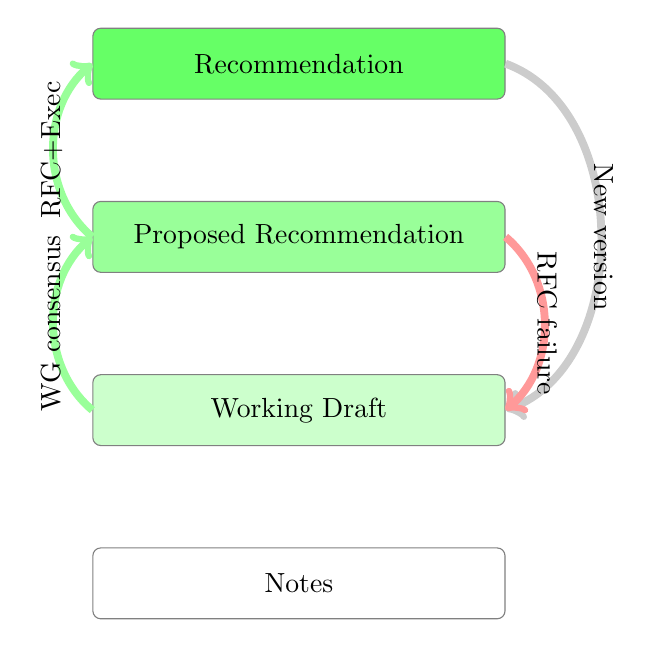
\begin{tikzpicture}[
status/.style={node distance=2.2cm, minimum height=0.9cm,
  rounded corners=1mm, thin,draw=black!50, text width=5cm,
  align=center},
procstep/.style={->, line width=1mm},
nodelabel/.style={color=black}]
\node (rec) [status, fill=green!60] {Recommendation};
\node (pr) [status, fill=green!40, below of=rec] {Proposed Recommendation};
\node (wd) [status, fill=green!20, below of=pr] {Working Draft};
\node (note) [status,below of=wd] {Notes};

\draw [procstep, bend left=50, color=green!40] (wd.west) to 
node[nodelabel,pos=0.5,rotate=90] {\strut WG consensus} 
(pr.west);

\draw [procstep, bend left=50, color=green!40] (pr.west) to 
node[nodelabel,pos=0.5,rotate=90] {\strut RFC+Exec} 
(rec.west);

\draw [procstep, bend left=70, color=black!20] (rec.east) to 
node[nodelabel,pos=0.5,rotate=270] {\strut New version} 
(wd.east);

\draw [procstep, bend left=50, color=red!40] (pr.east) to 
node[nodelabel,pos=0.5,rotate=270] {\strut RFC failure} 
(wd.east);


\end{tikzpicture}
\endgroup
